\section{Text to SQL}

\subsection{Foundational Evolution of Natural Language to SQL Parsing}
The translation of natural language queries (NL) into syntactically valid and semantically accurate Structured Query
Language (SQL) expressions---historically formalized as semantic parsing---has undergone distinct evolutionary paradigms
\cite{Multi_Agent_Collaborative_Framework_for_Text_to_SQL, Text_to_SQL_in_the_Era_of_LLMs}. Early technical
approaches relied entirely on rule-based statistical semantic parsers and deterministic translation patterns
\cite{Text_to_SQL_in_the_Era_of_LLMs}. These frameworks evaluated input streams at the token level, mapping
linguistic inputs directly onto rigid, single-table target database schemas via hardcoded template sketches or syntax
maps \cite{Text_to_SQL_in_the_Era_of_LLMs}. While computationally lightweight, these early systems lacked
scalability and generalizability, rendering them highly fragile when exposed to natural language synonyms, lexical
variations, or modified structural schemas \cite{Text_to_SQL_in_the_Era_of_LLMs}.


The field shifted significantly with the implementation of deep neural networks, specifically sequence-to-sequence
(Seq2Seq) neural architectures and Graph Neural Networks (GNNs) \cite{Text_to_SQL_in_the_Era_of_LLMs}. These
neural parsers substantially enhanced natural language intent understanding and vocabulary variation handling
\cite{Text_to_SQL_in_the_Era_of_LLMs}. To preserve structural validity during the generation phase, these
systems began utilizing Abstract Syntax Trees (AST) and structural decoders to ensure that the output adhered to
standard database syntax \cite{Multi_Agent_Collaborative_Framework_for_Text_to_SQL,
Text_to_SQL_in_the_Era_of_LLMs}.


The introduction of Pre-trained Language Models (PLMs) like BERT and T5 established the next major milestone,
drastically improving schema alignment and intent parsing \cite{Text_to_SQL_in_the_Era_of_LLMs}. PLM-driven
models achieved approximately 80\% accuracy on standard benchmarks like Spider 1.0
\cite{Text_to_SQL_in_the_Era_of_LLMs}. However, their performance deteriorated rapidly when exposed to
extra-hard query complexities or highly nested schema states \cite{Text_to_SQL_in_the_Era_of_LLMs}.


In the contemporary era of Large Language Models (LLMs), the task has been recast as an adaptive generation and
in-context execution problem \cite{Multi_Agent_Collaborative_Framework_for_Text_to_SQL,
Text_to_SQL_in_the_Era_of_LLMs}. Modern decoder-only and encoder-decoder architectures (e.g., GPT-4, Claude
3.5, and DeepSeek) leverage extensive parameters and emergence capabilities to analyze natural language logic and
database relations directly within the prompt context window, eliminating the need for rigid structural sketches or
decoding constraints \cite{Multi_Agent_Collaborative_Framework_for_Text_to_SQL, Text_to_SQL_in_the_Era_of_LLMs}.

\subsection{The Modular Pipeline Taxonomy in the LLM Era}
While classical Text-to-SQL translation was long treated as an end-to-end monolithic generation task, recent
advancements have enforced a highly structured, modular design pattern \cite{Text_to_SQL_in_the_Era_of_LLMs}. Modern systems
segment the Text-to-SQL lifecycle into three explicit execution phases: Pre-Processing, Core Translation, and
Post-Processing \cite{Text_to_SQL_in_the_Era_of_LLMs}.

\subsubsection{Pre-Processing Strategies}
The pre-processing stage is responsible for minimizing information noise and augmenting input text before it reaches the
language model backbone \cite{Text_to_SQL_in_the_Era_of_LLMs}. This phase consists of three core operational modules:

\begin{itemize}
   \item \textbf{Schema Linking:} This module isolates and maps specific natural language tokens to their corresponding structural items (tables and columns) within the database \cite{Text_to_SQL_in_the_Era_of_LLMs}. In early systems, this was achieved via exact or approximate string matching \cite{Text_to_SQL_in_the_Era_of_LLMs}. Modern systems deploy deep cross-encoders or specialized In-Context Learning (ICL) routines to dynamically score and rank structural elements by relevance, mitigating cross-domain vocabulary alignment gaps \cite{Text_to_SQL_in_the_Era_of_LLMs}.
   \item \textbf{Database Content Retrieval:} To satisfy literal filter constraints embedded in \texttt{WHERE} or \texttt{HAVING} clauses, systems must extract precise cell values from the physical database \cite{Text_to_SQL_in_the_Era_of_LLMs}. Because injecting whole database files into LLM prompts is structurally impossible, frameworks construct complex indexing and retrieval strategies \cite{Text_to_SQL_in_the_Era_of_LLMs}.
   \item \textbf{Additional Information Acquisition:} This module infuses external domain knowledge, formulaic definitions, metadata descriptions, and format constraints into the generation template \cite{Text_to_SQL_in_the_Era_of_LLMs}. This step prevents error propagation caused by a model's unfamiliarity with specialized corporate jargon or cross-domain rules \cite{Text_to_SQL_in_the_Era_of_LLMs}.
\end{itemize}

\subsubsection{Core Translation Frameworks}
The core translation layer handles the conversion of structured semantic contexts into executable relational code,
defined by specific encoding and decoding design choices \cite{Text_to_SQL_in_the_Era_of_LLMs}:

\begin{itemize}
   \item \textbf{Encoding Strategies:} Input serialization generally relies on \textit{Sequential Encoding}, where language queries, schema metadata, and inline comments are flattened into a single linear string \cite{Text_to_SQL_in_the_Era_of_LLMs}. Alternatively, \textit{Graph-Based Encoding} constructs highly interconnected graph abstractions that capture the physical database topology (e.g., primary-to-foreign key relationships), mapping them using Graph Attention Networks to explicitly preserve the schema design \cite{Text_to_SQL_in_the_Era_of_LLMs}.
   \item \textbf{Decoding Strategies:} Standard implementations leverage \textit{Greedy Search} or \textit{Beam Search} decoding paths \cite{Text_to_SQL_in_the_Era_of_LLMs}. However, advanced pipelines use \textit{Constraint-Aware Incremental Decoding} frameworks, such as PICARD \cite{Text_to_SQL_in_the_Era_of_LLMs}. These systems intercept token generation at each step, verifying the partial statement against the formal SQL grammar rules and schema-level constraints to prevent structural or syntactical errors before execution \cite{Text_to_SQL_in_the_Era_of_LLMs}.
   \item \textbf{Intermediate Representations (IR):} To mitigate the wide structural gap between unconstrained natural language and rigid SQL, architectures can translate queries into a grammar-free intermediate language \cite{Text_to_SQL_in_the_Era_of_LLMs}. Frameworks like NatSQL remove complex syntax components (such as implicit \texttt{FROM} and \texttt{JOIN} tables) to yield a simplified abstraction layer, which can later be deterministically expanded into database-specific SQL \cite{Text_to_SQL_in_the_Era_of_LLMs}.
\end{itemize}

\subsubsection{Post-Processing and Self-Correction}
Once an initial SQL statement is output by the model, post-processing layers are activated to check validity and execute
refinement loops \cite{Text_to_SQL_in_the_Era_of_LLMs}:

\begin{itemize}
   \item \textbf{Output Consistency and Voting:} To minimize model randomness, pipelines sample multiple execution paths simultaneously \cite{Text_to_SQL_in_the_Era_of_LLMs}. Frameworks use self-consistency voting or keyword clustering methods to select the most consistent candidate from the parallel generation runs \cite{Text_to_SQL_in_the_Era_of_LLMs}.
   \item \textbf{Execution-Guided Self-Correction:} This technique uses real-time runtime feedback to execute automated debugging loops \cite{Text_to_SQL_in_the_Era_of_LLMs}. By capturing execution states, syntax warnings, or empty result logs directly from the database server engine, the pipeline passes the raw error text back into specialized refinement blocks, mimicking human debugging processes \cite{Text_to_SQL_in_the_Era_of_LLMs}.
\end{itemize}

\subsection{Multi-Agent Collaboration and Role-Based Delegation}
The limits of monolithic, single-agent pipelines when exposed to massive enterprise schemas have driven the development
of multi-agent collaborative frameworks \cite{Multi_Agent_Collaborative_Framework_for_Text_to_SQL, SQLFixAgent_Towards_Semantic_Accurate_Text_to_SQL, Text_to_SQL_in_the_Era_of_LLMs}. Rather than forcing a
single LLM configuration to process the entire database state, reason through multi-hop questions, and write hundreds of
lines of dialect code, these frameworks assign specialized roles to distinct agents that collaborate via shared memory
contexts \cite{Multi_Agent_Collaborative_Framework_for_Text_to_SQL, SQLFixAgent_Towards_Semantic_Accurate_Text_to_SQL, Text_to_SQL_in_the_Era_of_LLMs}.

\begin{figure}[H]
   \centering
   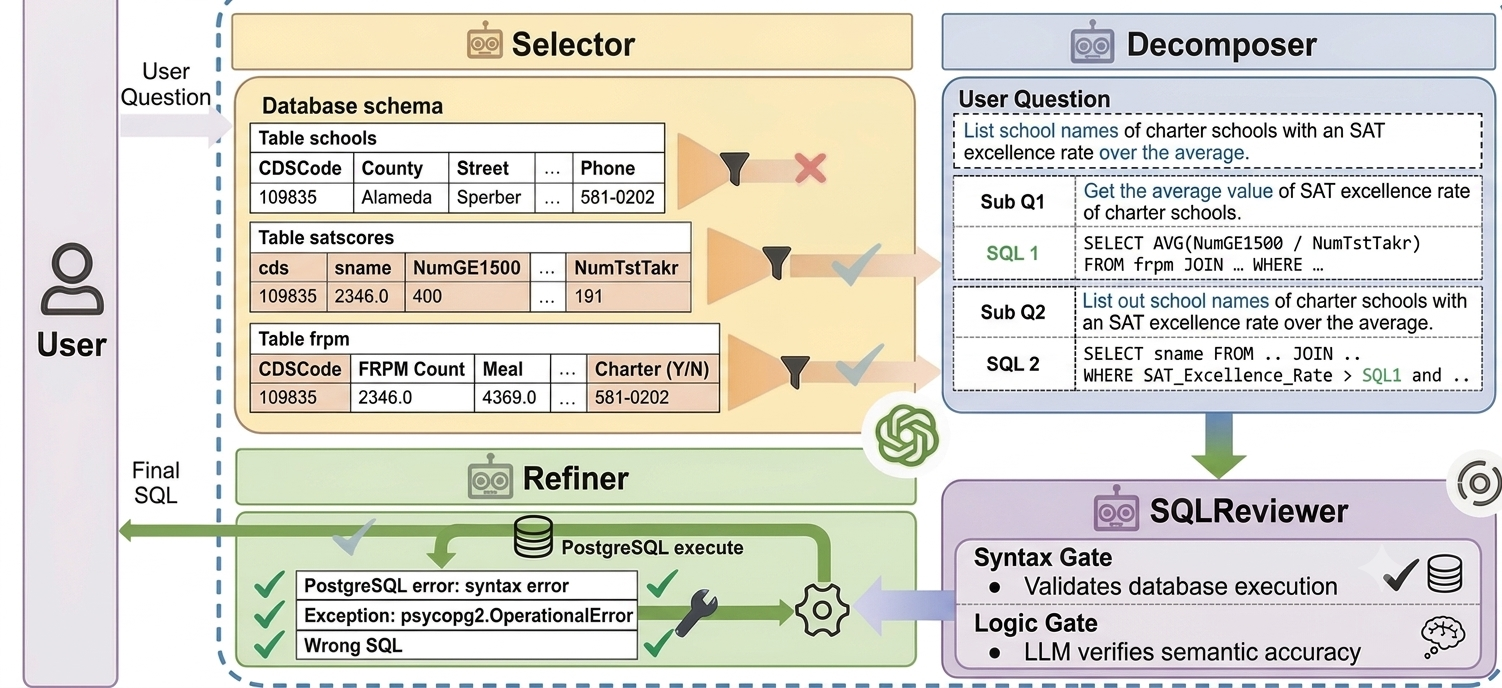
\includegraphics[width=\linewidth,height=0.9\textheight,keepaspectratio]{images/ai/text2SQL.png}
   \caption{Multi-Agent Pipeline}
   \label{fig:Multi-Agent Pipeline}
\end{figure}

\subsubsection{The Schema Linker (Selector Agent)}
The Selector agent handles the task of schema linking and prompt optimization \cite{Multi_Agent_Collaborative_Framework_for_Text_to_SQL, Text_to_SQL_in_the_Era_of_LLMs}.
When exposed to real-world industrial environments containing hundreds of tables and thousands of columns, injecting the
complete data description creates severe information interference, misleads column matching, and incurs unsustainable
API token costs \cite{Multi_Agent_Collaborative_Framework_for_Text_to_SQL, Text_to_SQL_in_the_Era_of_LLMs}. The Selector isolates a minimal relevant sub-schema based on
semantic similarity to the user's question \cite{Multi_Agent_Collaborative_Framework_for_Text_to_SQL, Text_to_SQL_in_the_Era_of_LLMs}. It drops irrelevant tables and
retains a strictly bounded column footprint per table---ensuring that the subsequent generation layers receive a clean,
high-density context prompt \cite{Multi_Agent_Collaborative_Framework_for_Text_to_SQL}.

\subsubsection{The Logic Decomposer}
For complex analytical questions requiring nested subqueries, common table expressions (CTEs), or multi-table joins,
single-pass generation frequently falls into reasoning traps \cite{Multi_Agent_Collaborative_Framework_for_Text_to_SQL, TEXT_TO_SQL_WORKFLOWS, Text_to_SQL_in_the_Era_of_LLMs}. The
Decomposer agent handles task breakdown by fracturing the natural language question into a sequence of simpler,
executable sub-questions \cite{Multi_Agent_Collaborative_Framework_for_Text_to_SQL, Text_to_SQL_in_the_Era_of_LLMs}. Operating via sequential Chain-of-Thought (CoT) logic,
it builds sub-SQL components progressively \cite{Multi_Agent_Collaborative_Framework_for_Text_to_SQL, Text_to_SQL_in_the_Era_of_LLMs}. The execution output or logical
structure of an early subquery serves as the structural foundation for the next analytical block, ensuring that each
component is validated before final assembly \cite{Multi_Agent_Collaborative_Framework_for_Text_to_SQL}.

\subsubsection{The Semantic Reviewer and Refiner}
A critical vulnerability in modern implementations is the semantic consistency gap: models frequently output
syntactically clean SQL queries that execute perfectly without throwing database errors, but return incorrect data
because the query logic does not align with the user's actual intent \cite{SQLFixAgent_Towards_Semantic_Accurate_Text_to_SQL, Text_to_SQL_in_the_Era_of_LLMs}. To
address this, current research integrates a dual-agent check system:

\begin{figure}[ht]
\centering
\begin{verbatim}
              +--------------------------------+
              |  Generated SQL from Decomposer |
              +---------------+----------------+
                              |
                              v
              +--------------------------------+
              |    Gate 1: Database Engine     |
              |     (Execution Sanity Check)   |
              +---------------+----------------+
                              |
                    +---------+---------+
                    |                   |
              [Passes Check]      [Fails Check]
                    |                   |
                    v                   v
    +-------------------------------+   |
    |     Gate 2: SQLReviewer       |   |
    |  (Rubber Duck Debugging)      |   |
    +---------------+---------------+   |
                    |                   |
          +---------+---------+         |
          |                   |         |
     [Logically]         [Logical]      |
      [Correct]          [Mismatch]     |
          |                   |         |
          v                   v         v
  +---------------+   +---------------------------+
  | Final Correct |   |   SQLRefiner Agent Loop   |
  |   SQL Output  |   | (Failure Memory/ICL)      |
  +---------------+   +-------------+-------------+
\end{verbatim}
\caption{Dual-Gate Verification and Refinement Flow}
\end{figure}

The SQLReviewer agent is engineered for latent semantic error detection \cite{SQLFixAgent_Towards_Semantic_Accurate_Text_to_SQL}. It adopts the
software engineering principle of \textit{Rubber Duck Debugging}, systematically parsing and explaining the generated
SQL code block line-by-line to evaluate whether the joins, selections, and filters precisely match the user's intent
\cite{SQLFixAgent_Towards_Semantic_Accurate_Text_to_SQL}. If a logical conflict or execution crash is flagged, the query is passed to the SQLRefiner
agent \cite{SQLFixAgent_Towards_Semantic_Accurate_Text_to_SQL}. The Refiner acts as an automated debugging engine, utilizing failure memory
reflection and logging historical execution history to iteratively correct the SQL statement until it successfully
passes through both validation gates \cite{SQLFixAgent_Towards_Semantic_Accurate_Text_to_SQL, Text_to_SQL_in_the_Era_of_LLMs}.

\subsection{Architectural Calibration: Fine-Tuning vs. In-Context Learning}
Deploying Text-to-SQL capabilities within corporate settings requires careful optimization across training and inference
dimensions \cite{Text_to_SQL_in_the_Era_of_LLMs, Optimizing_text_to_SQL}. Recent engineering studies from 2025 highlight the major
performance and structural trade-offs between zero-shot/few-shot In-Context Learning (ICL) and domain-specific
Supervised Fine-Tuning (SFT) \cite{Text_to_SQL_in_the_Era_of_LLMs, Optimizing_text_to_SQL}.

\subsubsection{Evaluation Benchmarks and Metrics}
System calibration and model accuracy are measured using two standardized evaluation parameters \cite{Text_to_SQL_in_the_Era_of_LLMs,
Optimizing_text_to_SQL}:
\begin{enumerate}
   \item \textbf{Valid Efficiency Score (VES):} Evaluates the computational efficiency of the generated SQL queries. Unlike basic accuracy metrics, VES measures the execution time and resource optimization of the model-generated query relative to the ground-truth SQL. This metric ensures that the system produces not only semantically correct but also highly performant code suitable for massive production environments \cite{Text_to_SQL_in_the_Era_of_LLMs, Optimizing_text_to_SQL}.
   \item \textbf{Execution Accuracy (EX):} Measures the precise proportion of generated queries that return a data result identical to the ground-truth query when executed against the physical target database \cite{Text_to_SQL_in_the_Era_of_LLMs, Optimizing_text_to_SQL}.
\end{enumerate}

\subsubsection{Trade-offs and the ``Inverse-Skilled Bias''}
Empirical model evaluations establish distinct trade-offs between closed-source API prompting and local fine-tuning
\cite{Text_to_SQL_in_the_Era_of_LLMs, Optimizing_text_to_SQL}:

% \begin{table}[h]
% \centering
% \begin{tabular}{|p{0.2\textwidth}|p{0.25\textwidth}|p{0.25\textwidth}|p{0.1\textwidth}|p{0.15\textwidth}|}
% \hline
% \textbf{Optimization Strategy} & \textbf{Pros} & \textbf{Cons} & \textbf{Data Privacy} & \textbf{Resource Requirements} \\
% \hline
% \textbf{In-Context Learning (ICL)} (e.g., GPT-4, Claude 3.5) & Zero retraining time; rapid adaptation via prompt changes; elite general reasoning \cite{Text_to_SQL_in_the_Era_of_LLMs, Optimizing_text_to_SQL}. & High token consumption; volatile prompt sensitivity; extreme API costs at scale \cite{Text_to_SQL_in_the_Era_of_LLMs, Optimizing_text_to_SQL}. & Low (Exposes queries to external servers) \cite{Text_to_SQL_in_the_Era_of_LLMs}. & High API budget; zero local hardware overhead \cite{Text_to_SQL_in_the_Era_of_LLMs, Optimizing_text_to_SQL}. \\
% \hline
% \textbf{Supervised Fine-Tuning (SFT)} (e.g., Specialized open models) & Captures deep structural domain context; stable schema mapping; near-zero prompt overhead \cite{Text_to_SQL_in_the_Era_of_LLMs, Optimizing_text_to_SQL}. & Requires high-quality, human-curated training pairs; risk of overfitting baseline text patterns \cite{Multi_Agent_Collaborative_Framework_for_Text_to_SQL, Text_to_SQL_in_the_Era_of_LLMs}. & High (Enables fully air-gapped, local deployment) \cite{Text_to_SQL_in_the_Era_of_LLMs}. & Local GPU clusters required for initial parameters calibration \cite{Text_to_SQL_in_the_Era_of_LLMs}. \\
% \hline
% \end{tabular}
% \caption{Strategic Trade-offs between ICL and SFT}
% \end{table}
% %%%%%%%%%%%%%%%%%%%%%%%%%%%%%%%%%%%%%%%%%%%%%%%%%%%%%%%5
% \begin{table}[ht]
% \centering
% \small
% \caption{Strategic Trade-offs between ICL and SFT}
% \label{tab:icl_sft_comparison}

% \begin{tabularx}{\textwidth}{|p{2.8cm}|X|X|p{1.8cm}|p{2.2cm}|}
% \hline
% \textbf{Optimization Strategy} &
% \textbf{Pros} &
% \textbf{Cons} &
% \textbf{Data Privacy} &
% \textbf{Resource Requirements} \\
% \hline

% \textbf{In-Context Learning (ICL)}
% (e.g., GPT-4, Claude 3.5)
% &
% Zero retraining time, rapid adaptation through prompt engineering, and strong general reasoning capabilities \cite{Text_to_SQL_in_the_Era_of_LLMs,Optimizing_text_to_SQL}.
% &
% High token consumption, prompt sensitivity, and significant API costs at scale \cite{Text_to_SQL_in_the_Era_of_LLMs,Optimizing_text_to_SQL}.
% &
% Low; queries are processed on external servers \cite{Text_to_SQL_in_the_Era_of_LLMs}.
% &
% High API expenditure but no local hardware requirements \cite{Text_to_SQL_in_the_Era_of_LLMs,Optimizing_text_to_SQL}.
% \\
% \hline

% \textbf{Supervised Fine-Tuning (SFT)}
% (e.g., specialized open-source models)
% &
% Learns domain-specific structures, provides stable schema mapping, and minimizes prompt overhead \cite{Text_to_SQL_in_the_Era_of_LLMs,Optimizing_text_to_SQL}.
% &
% Requires high-quality training data and may overfit to training patterns \cite{Multi_Agent_Collaborative_Framework_for_Text_to_SQL,Text_to_SQL_in_the_Era_of_LLMs}.
% &
% High; supports fully local and air-gapped deployment \cite{Text_to_SQL_in_the_Era_of_LLMs}.
% &
% Requires GPU resources during training but has lower inference costs afterward \cite{Text_to_SQL_in_the_Era_of_LLMs}.
% \\
% \hline

% \end{tabularx}
% \end{table}
% %%%%%%%%%%%%%%%%%%%%%%%%%%%%%%%%%%%%%%%%%%%%%%%%%%%%%%%5
% \begin{table}[ht]
% \centering
% \small
% \caption{Strategic Trade-offs between ICL and SFT}
% \label{tab:icl_sft_comparison}

% \renewcommand{\arraystretch}{1.4}

% \begin{tabularx}{\textwidth}{p{3cm} X X p{2.5cm} p{2.8cm}}
% \toprule
% \textbf{Optimization Strategy} &
% \textbf{Pros} &
% \textbf{Cons} &
% \textbf{Data Privacy} &
% \textbf{Resource Requirements} \\
% \midrule

% \textbf{In-Context Learning (ICL)}

% \textit{(e.g., GPT-4, Claude 3.5)}
% &
% Zero retraining time; rapid adaptation via prompt changes; elite general reasoning.
% &
% High token consumption; volatile prompt sensitivity; extreme API costs at scale.
% &
% Low (Exposes queries to external servers).
% &
% High API budget; zero local hardware overhead.
% \\[0.8em]

% \textbf{Supervised Fine-Tuning (SFT)}

% \textit{(e.g., Specialized open models)}
% &
% Captures deep structural domain context; stable schema mapping; near-zero prompt overhead.
% &
% Requires high-quality, human-curated training pairs; risk of overfitting baseline text patterns.
% &
% High (Enables fully air-gapped, local deployment).
% &
% Local GPU clusters required for initial parameter calibration.
% \\

% \bottomrule
% \end{tabularx}
% \end{table}
% %%%%%%%%%%%%%%%%%%%%%%%%%%%%%%%%%%%%%%%%%%%%%%%%%%%%%%%5
\begin{table}[ht]
\centering
\small
\caption{Strategic Trade-offs between ICL and SFT}
\label{tab:icl_sft_comparison}

\renewcommand{\arraystretch}{1.4}

% The >{\raggedright\arraybackslash} command forces left-alignment 
% and completely eliminates the stretched word spacing.
\begin{tabularx}{\textwidth}{
    >{\raggedright\arraybackslash}p{3cm} 
    >{\raggedright\arraybackslash}X 
    >{\raggedright\arraybackslash}X 
    >{\raggedright\arraybackslash}p{2.5cm} 
    >{\raggedright\arraybackslash}p{2.8cm}
}
\toprule
\textbf{Optimization Strategy} &
\textbf{Pros} &
\textbf{Cons} &
\textbf{Data Privacy} &
\textbf{Resource Requirements} \\
\midrule

\textbf{In-Context Learning (ICL)} \newline
\textit{(e.g., GPT-4, Claude 3.5)}
&
Zero retraining time; rapid adaptation via prompt changes; elite general reasoning.
&
High token consumption; volatile prompt sensitivity; extreme API costs at scale.
&
Low (Exposes queries and metadata to external servers).
&
High API budget; zero local hardware overhead.
\\[0.8em]

\textbf{Supervised Fine-Tuning (SFT)} \newline
\textit{(e.g., Specialized open models)}
&
Captures deep structural domain context; stable schema mapping; near-zero prompt overhead.
&
Requires high-quality, human-curated training pairs; risk of overfitting baseline text patterns.
&
High (Enables fully air-gapped, local deployment).
&
Local GPU clusters required for initial parameter calibration.
\\

\bottomrule
\end{tabularx}
\end{table}

\subsection{Frontier Challenges: Real-World Enterprise Workflows}
While traditional models achieved high scores on classic benchmarks like Spider 1.0 (91.2\%) and BIRD (73.0\%), recent
2025 research reveals that these platforms struggle when deployed within true corporate production environments
\cite{TEXT_TO_SQL_WORKFLOWS}. The introduction of the \textbf{Spider 2.0} benchmark highlights a massive complexity gap
between academic configurations and industrial database operations \cite{TEXT_TO_SQL_WORKFLOWS}.

\subsubsection{Real-World Schema and Architecture Traits}
Production-grade systems differ from academic benchmarks across several key areas \cite{TEXT_TO_SQL_WORKFLOWS}:
\begin{itemize}
   \item \textbf{Scale and Scope:} Production databases move away from small, clean, local tables, transitioning to terabyte-scale cloud data lakes (e.g., Google BigQuery, Snowflake) characterized by massive schemas that frequently contain over 1,000 columns across nested relational structures \cite{TEXT_TO_SQL_WORKFLOWS}.
   \item \textbf{Nested Records and Unstructured Fields:} Industrial systems frequently abandon flat tables, storing complex data in nested \texttt{STRUCT} arrays, spatial geography points, or loose \texttt{JSON} objects directly within a single column \cite{TEXT_TO_SQL_WORKFLOWS}. Models cannot resolve these schemas via standard column linking, requiring multi-step extraction reasoning and specialized dialect function mapping \cite{TEXT_TO_SQL_WORKFLOWS}.
   \item \textbf{Dialect Divergence:} Production applications require navigating subtle, platform-specific syntax nuances across diverse database engines---including SQLite, DuckDB, PostgreSQL, ClickHouse, and Snowflake \cite{TEXT_TO_SQL_WORKFLOWS}. This variance demands that agents dynamically query platform documentation to extract specific analytical functions (e.g., \texttt{DATE\_TRUNC} or \texttt{ST\_DISTANCE}) to match regional data constraints \cite{TEXT_TO_SQL_WORKFLOWS}.
\end{itemize}